\chapter{Problem Analysis}\label{ch:problemanalysis}
In this chapter, we delwe deeper into the problem stated in \cref{ch:introduction}. While the eventual solution is aimed at the area of modular factories as a whole, we use the FESTO modular factory system \cite{FESTOweb} as a point of reference. This system was chosen specifically as Aalborg University's \textit{Department of Mechanical and Manufacturing Engineering} have an existing set-up, which we were allowed to inspect. 

\section{FESTO}\label{sec:festo}
The FESTO system accessible to us is the Cyber-Physcial(CP) Learning Factory. This is not intended for full fledged production, but rather it is used in education and research. While not an industrial system, we deem that it will aid in a general understanding of the field and its related problems. The public litterature about the CP Learning factory is rather light. The most reliable sources come from FESTO themselves, as in the case with \cite{CPFactory2015}. To supply the written material, we also use our own observations about the local set-up, in addition to statements made by staff working the factory.  

\begin{figure}[h]
\centering
\includegraphics[width=\textwidth]{CP_Factory.jpg}
\caption{A CP-factory setup}
\label{fig:festo-example}
\end{figure}

An example of a CP-factory set-up can be seen in \cref{fig:festo-example}. Each module in a set-up is made up of the same base module. This includes a control panel as well as two conveyor belts moving in opposite directions. Modules can be connected either at the narrow ends or on the face opposite the control panel. On each module new equipment may be fitted. This can include a robot arm, a drill or a camera. A module works only on one item at a time. Yet several items may be located on the same module, being queued up and waiting to be worked on or pass through the module.

The factory control tasks are handled through a MES(Manufacturing Execution System)known as MES4. This controls production order dispatch, scheduling, resource management etc. During production the MES4 system signals individual modules to perform certain actions. These instructions are encoded into the module's own controller as KRL code.

The factory also uses a large amount of networking technologies. RFID technology is used to monitor the location of individual items running along the conveyor belts. Individual modules may communicate by field-bus, while overall communications in the factory occurs over a WLAN. The factory may also be connected to an Enterprise Resource Planning (ERP) system or other factories through MES4. A production run is initiated by activating each module through its control panel, then launching from a PC.

\section{Problems in modular factories}
Through our discussion with staff at Aalborg University we identified some problems relating to use of the CP Learning Factory. Additional problems concerning modular factories in general were found by looking into the literature. In this section we will examine each of these issues. 

\subsection{Calculating an optimal factory configuration}
Aalborg staff relayed to us that they would like to generate optimal factory configurations according to some order of items, which must be produced. A configuration is here the same as the layout of a factory, which considers where modules are placed, and which other modules they connect to.

Product Lifecycle Management (PLM) systems such as Siemens' Technomatix \cite{Siemens2014} have this sort of functionality included. Technomatix is able to simulate factories and their throughput before implementation. Yet, the system does not focus on rapidly changing factory configurations. It concerns itself with getting the configuration right before implementation. When new orders come in, Technomatix may suggest how to optimize production parameters for an implemented configuration. This may entail an alteration in how production is scheduled. A production schedule informs us, how we should produce an order of items using a specefic configuration. Manufacturers are interested in finding the schedule, which delivers the the highest throughput of items in an order on a given configuration. 

As Technomatix is more about altering parameters of current factory configurations, it is not a good fit when working with modular factories. In a modular factory system, the factory configuration may be altered in response to a new order of items. The problem is not only about finding the fastest schedule on an already implemented configuration. It also concerns looking at alternative configurations, and seeing if any of these have an even better schedule. We may also deal with the cost of moving from one configuration to the next. Even though one configuration may be very efficient, it may be expensive to reconfigure the current configuration in order to set it up. 

\subsection{Manual Software Reconfiguration}
On the issue of reconfiguration, Aalborg staff informed us that the difficult part of setting up a new factory configuration is not the moving and connecting of the physical modules. Instead it is the alterations made to individual modules. As mentioned in \cref{sec:festo}, each module has a set of instructions encoded in KRL code, which the MES4 system may signal for them to accomplish. As a factory is reconfigured this code will most likely have to be changed. This is no light task, as there must be an instruction for each case in which MES4 system may signal the module. If a red phone has to be treated differently from a black phone, there needs to be a separate instruction. Programmers have to handle each mundane case, leading to a lot of boilerplate code. 

The staff here at Aalborg themselves, suggested that they would like a way to generate the KRL code. This problem is of course not only relevant in the case of FESTO. Any production line has to update its machine controlling code, if it reconfigures its layout.

\subsection{Security}
Like with the rest of Industry 4.0, modular factories rely heavily on networking technologies to interconnect every part of production. Through this network a lot of security and safety-critical data is send. According to Sadeghi\cite{Sadeghi2015}, security is often not adequate and modular factories are thus at risk of infiltration from many different angles. This is an issue, as an attack on a modular factory risks both monetary, but also human loss. Yet, it also seems that many modern security methods do not work for the modular factory. This is in part because a factory has a high requirement for availability. Thus a registered attack can not simply be countered by halting production. In addition, modules are often required to have low power consumption and minimal cost. Again, security features will clash with these requirements. 

\subsection{Big Data}
Modular factories store a lot of data about their production. Each individual module, item and piece of equipment may be a source of information. Thus there is a vast amount of heterogeneous data to deal with. We must concern the field of Big Data, the challenges it brings along. Yin \cite{Yin2015} mentions that the size of data itself puts significant requirements on both hardware and software. He also states that there is an issue of how to use the data for real time analysis and detection. Not all data is interesting either, so the cleaning of raw data has to be handled as well. 

\section{A running factory example}\label{sec:runningexample}
In this section we set up an example of a factory, which we will refer to throughout the report. It can be seen on \cref{fig:running-example}. It depicts a specific factory configuration for producing various children's toys. We use this example to present some of the core concepts used in this report. In the final part of this report, we will try to generate this configuration, given only its modules and an order of items it needs to produce. In this section we will also discuss, what parts of the real world we choose to model.

\begin{figure}[h]
\centering
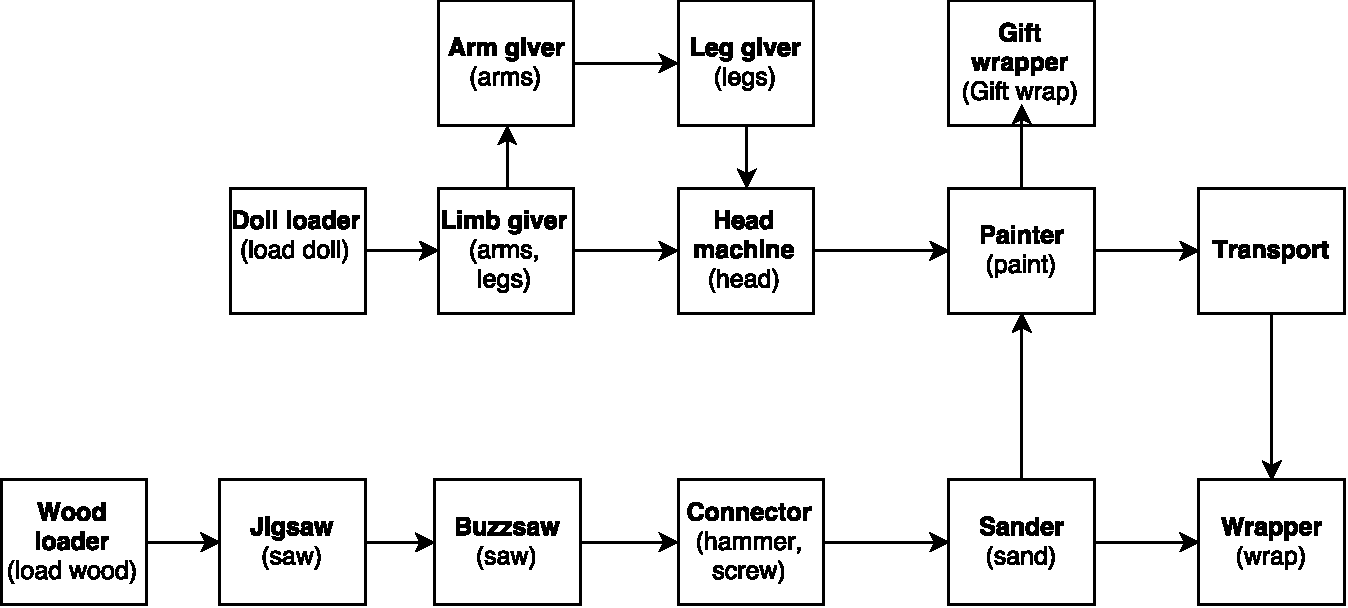
\includegraphics[width=\textwidth]{runningexample.pdf}
\caption{An example of a toy factory layout}
\label{fig:running-example}
\end{figure}

\subsection{Modules}
On the diagram, we have chosen to depict a module as a square, which may connect to other modules. Each module has a name, shown in bold. A module may perform one or more types of work upon an item, these are shown in parenthesis. Each work type takes a certain amount of time to complete. It also takes a certain amount of time for an item to be transported through a module. A module may only work on one item at a time. These are all properties, which we discovered by inspecting the CP learning factory.

A connection signifies, how we may pass items between modules. There are real world physical restrictions upon these connections, in that each module may only connect to at most four other modules. At the same time, a module can only connect to another module, if they are placed right next to each other. On the diagram, we have chosen to move the modules away from each other to fit the arrows, but in the physical layout connected modules lay side by side. Yet, just because modules are placed next to each other, does not mean there needs to be a connection. 

We choose to restrict connections in this way as modules tend to be rectangular in shape as in the case of the CP Learning Factory. We also allow only one neighbour per side, restricting us to four connections total. In reality the modules in the CP Learning Factory leave one side open for a control panel, so only three neighbours are allowed. We choose to look away from this requirement, as this may not be the case for all real life modules. CP Learning Factory modules also have two seperate conveyor belts on each module. We instead imagine a single conveyor per module from which we may guide items to all sides of the module. In addition, we choose to view our modules as square, while the CP Learning Factory modules are only rectangular. Modules from different systems may have many different shapes, so we choose the one, which is easiest to work with, when we later have to deal with modelling the physical placement of modules. If we need to model non-square modules, we must add their properties to the rule set, which guides placement. 

If we wish to connect two modules, which are not neighbours, we may connect them through one or more transport modules. This is a type of module that does not perform any type of work on items, other than ferrying them along a conveyor. On the diagram, a transporter is used to connect the \textit{Painter} and \textit{Wrapper} modules. Yet, using transport modules we can not freely connect any two modules, as the transporters have to be physically placeable. That is, they may physically not intersect any other module. This is the case when placing down any type of module. We view the factory layout on a 2-dimensional plane, where each module has the same height. This means that two modules intersect, if they take up the same space on this plane. We choose to disregard the third dimension, as modules tend to be of equal height.  

\subsection{Items}
In our factory, various items may be produced. The top line is used to produce dolls, while the bottom is used to produce toys made of wood, such as wooden swords. 

A doll needs to have its base loaded onto the factory. Then it needs to have arms, legs and head attatched, followed by a layer of paint and finally a gift wrapping. This set of linearly dependent instructions is called a recipe. It describes, how we may create items of a specefic type. Several identical items may be constructed to the same recipe. A recipe also indicates, the module at which items should begin production. In this case it would be \textit{Doll loader}. To complete a doll according to this recipe, we may have the doll base worked on by the following sequence of modules \textit{Doll loader}, \textit{Limb giver}, \textit{Head machine}, \textit{Painter} and \textit{Gift wrapper}. This sequence provides the types of work needed in the order specified by the recipe. Once an item has fulfilled its recipe it is removed from the factory. 

A wooden sword may have a recipe, which says that it first needs to have wood loaded onto the factory. Followed by sawing, hammering, sanding, painting and finally regular wrapping. It needs to start in \textit{Wood Loader}. To make a sword, we may work using the following sequence of modules: \textit{Wood}, \textit{Loader}, \textit{Jigsaw}, \textit{Connector}, \textit{Sander}, \textit{Painter} and \textit{Wrapper}. Notice that the sword will have to use the transport module to get wrapped. We could also have connected the \textit{Wrapper} directly to the \textit{Painter}. However that would require wooden items that do not require painting, such as a rocking horse, to pass through the \textit{Painter} module in order to get wrapped. The best placement depends on many factors such as the speed of individual modules, and how many wooden swords need to be produced in proportion to the amount of rocking horses.

\subsection{Parallelism}
Many items can obivously be worked on in parallel by the many modules of the factory. However we would like to focus on a specific type of parallel production, which increases throughput. We want items made according to the same recipe and having reached the same point in production to be worked on concurrently by different modules.  

On the bottom line, we do not need both \textit{Jigsaw} and \textit{Buzzsaw} modules to produce wooden items according to the shown recipes. One is enough. However, in the case that we need to produce many wooden swords, it may be beneficial to have both modules, as we can then double the rate, at which we can saw our wood. This of course requires that wood may pass through the \textit{Jigsaw} module, while it is sawing, in order to reach the \textit{Buzzsaw}.

On the top line we have an off-branching line consisting of \textit{Arm giver} and \textit{Leg Giver}. Again, these are not required to produce dolls. Yet, by adding this branch, we allow for two doll bases to have arms and legs added at the same time. This increases the throughput of dolls. We may choose to parallelize execution in this manner, as opposed to the previous way, if we do not wish to lengthen the current production line. It may also be used, if we want to parallelize a module's work, but we may not pass through that module, while it is working, as we can with \textit{Jigsaw}.

Aalborg staff have not set up their factory to enable this type of parallel production. Yet they state that they would do so to increase throughput, if they had the additional modules to do so. 

\section{Problem Definition}\label{ch:problemdefinition}
This report started by bringing up Industry 4.0 in addition to the modular factory. This lead to the following initial problem:

\bigskip
\textit{How may it be possible to optimize the throughput of individual production lines in a modular factory system, while keeping down the overall cost of production?}
\bigskip

Afterwards we looked deeper into the field of modular factories, using FESTO's CP Learning Factory as a starting point. From this we found a few challenges that modular factories are facing. Some relate to industry 4.0 as a whole, such as handling security and Big Data. Looking at the issues facing modular factories in particular, we see that the main problem lies in reconfiguration, as it requires a lot of resources. This is somewhat surprising, since modular factories are mainly based on frequent reconfiguration. In addition we have provided a running example of a factory configuration, and already discussed what properties of the real world modular factories, we wish to model.

For this project, we choose to concern ourselves with the issue of producing optimal factory configurations, given some order of items that needs to be produced and a set of avaliable modules. We define an optimal configuration to be the factory layout, which has the fastest schedule, and thus the highest throughput, among all candidate configurations. We formulate the goal of this project with the following project statement:

\bigskip
\textit{How may we, given some order of items and set of avaliable modules, be able to generate a factory configuration which has the fastest schedule of any other candidate configuration?}
\bigskip

This problem is solved in two parts. The first will concern itself with the actual modelling and simulation of a modular factory. This should allow us to simulate any factory configuration, and allow us to generate its fastest schedule for producing a given order. We rate a configuration according to the time taken to execute its fastest schedule. The second part of the solution will concern, how we pick the optimal configuration by generating candidates and comparing their ratings as to identify the optimal one. 


